%*****************************************************************
%*************************** Section 7 ***************************
%**************** Streckenerkennung des Fahrzeugs ****************
%*****************************************************************


\pagestyle{fancy}
\rhead{\thepage} \chead{} \lhead{\ref{Sec7}. \nameref{Sec7}}
\cfoot{}

\section{Streckenerkennung des Fahrzeugs}\label{Sec7}

Für die Streckenerkennung des Fahrzeugs stehen zwei Kamera-Typen zur Verfügung. Zum einen kann die Pixy2 Kamera verwendet werden, welche eine Auflösung von 640x400 Bildpunkten besitzt. Die andere Möglichkeit ist eine einfache Zeilenkamera mit einer Auflösung von 1x128 Bildpunkten.\vspace{11pt}

Da in vorherigen Projekten meist die Zeilenkamera verwendet wurde, wird für dieses Projekt dieselbe eingesetzt. Ein Grund dafür ist, dass die Verwendung von Bildern von so großer Auflösung, wie bei der Pixy2 Kamera, viel Rechenressourcen und Zeit kostet. Eine geringere Auflösung ist deshalb für die Schnelligkeit des Fahrzeugs von großer Wichtigkeit. \vspace{11pt}

Da mehr als eine Kamera am Fahrzeug erlaubt ist, kann bei der Weiterführung des Projekts natürlich die Funktion einer weiteren Kamera implementiert werden. Sinnvoll kann das vor allem dann sein, wenn die additive Kamera im Gegensatz zur Zeilenkamera auf der Strecke weiter voraussieht, um Streckenverlaufs-Änderungen früher zu erkennen. Auch bei Kreuzungen, an denen die Seitenlinien kurz verschwinden, kann eine zweite Kamera dabei helfen, den Streckenverlauf nicht zu verlieren.

\subsection{Kamera des Fahrzeugs}\label{Sec7Sub1}

Wie in der Einführung dieses Kapitels bereits erwähnt, wird eine Zeilenkamera mit einer Auflösung von 1x128 Bildpunkten verwendet (TAOS TSL1401R-LF). Die Kamera kann mit einer maximalen Taktfrequenz von 8MHz betrieben werden.

\begin{figure}[H] %H für Positionierung hier
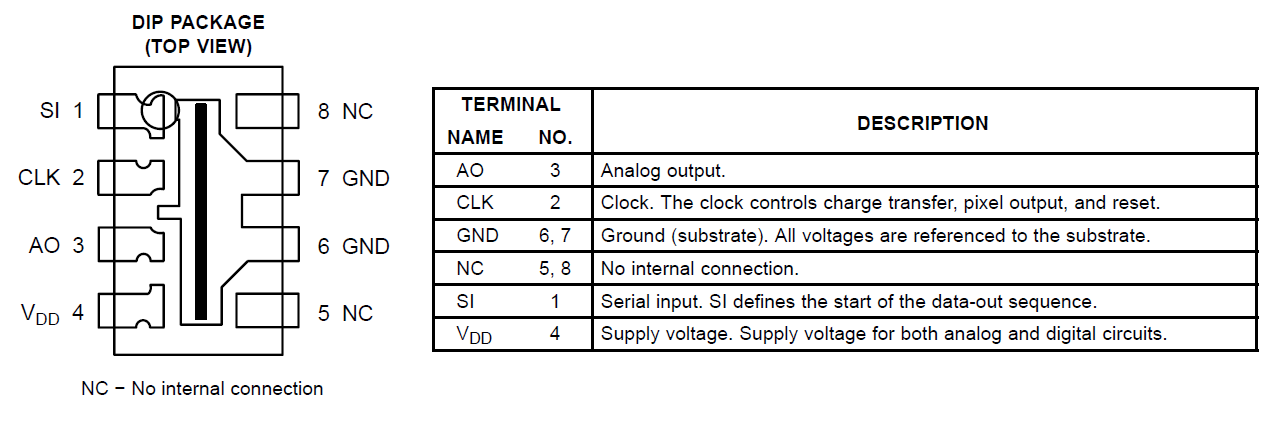
\includegraphics[width=.90\textwidth]{sec7/images/CamPinning} 
\centering
\captionsetup{width=.95\textwidth}
\caption[Pinbelegung der Taos Zeilenkamera TSL1401R-LF ~\protect\cite{Taos}]{Pinbelegung der Taos Zeilenkamera TSL1401R-LF ~\protect\cite{Taos}}\centering
\label{fig:CamPinning}
\end{figure}

In Abbildung \ref{fig:CamPinning} ist die Anschlussbelegung des Kamerachips und in Abbildung \ref{fig:CamWaveform} der zeitliche Verlauf eines Bildtransfers aus Sicht der Kamera abgebildet. Je höher die Taktfrequenz der Kamera-Clock (CLK), desto schneller kann eine einzelne Aufnahme getätigt werden (Bildaufnahmegeschwindigkeit). Der serielle Eingang der Kamera (SI) startet die Aufnahme. Damit die Kamera das Startsignal erkennt, muss dieses mindestens 20ns vor der steigenden Flanke der Kamera-Clock anliegen (t\textsubscript{su(SI)}, \glqq{}Setup time, serial input\grqq{}). Da die \glqq{}Hold time\grqq{} des seriellen Eingangs (t\textsubscript{h(SI)}) im Datenblatt 0ns beträgt, kann sich das Rücksetzen des SI-Signals gleichzeitig mit der Clock-Flanke ereignen. Je Clock-Zyklus wird ein einzelnes Pixel ausgelesen. Für die ADC-Messung ist unbedingt die \glqq{}Settling Time\grqq{} zu beachten (t\textsubscript{ts}), vor deren Ablauf der ADC nicht getriggert werden darf. Die Sampling-Zeit muss im Gegensatz zur Konversion vor Beginn des nächsten Clock-Zyklus zu Ende sein. Die Konversion hingegen hat Zeit bis zum nächsten ADC Trigger. Die Clock-Frequenz wird also von der Dauer einer ADC-Konversion beschränkt und nicht durch die technische Grenze von 8MHz. 

\begin{figure}[H] %H für Positionierung hier
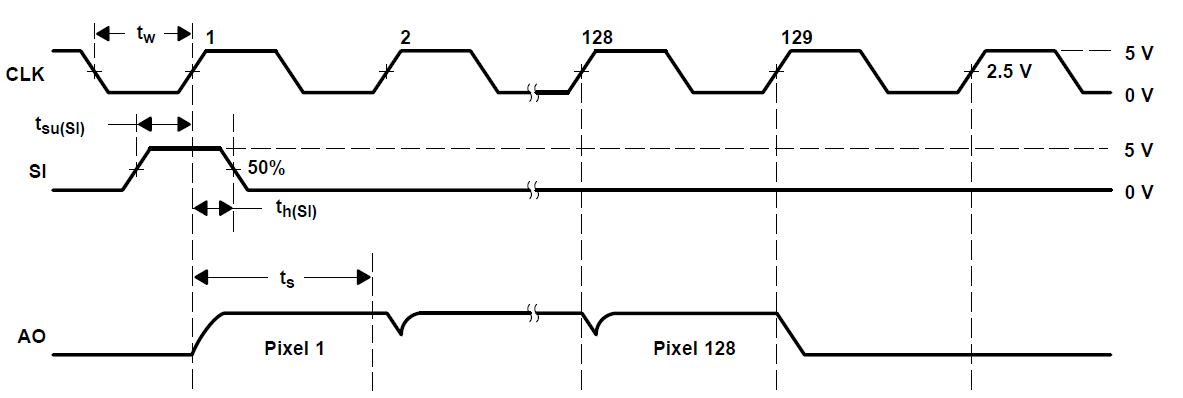
\includegraphics[width=.95\textwidth]{sec7/images/CamWaveform} 
\centering
\captionsetup{width=.95\textwidth}
\caption[Zeitverlauf einzelner Pixeltransfers aus Sicht der Kamera ~\protect\cite{Taos}]{Zeitverlauf einzelner Pixeltransfers aus Sicht der Kamera TSL1401R-LF  relativ zur vom Controller bereitgestellten Kamera-Clock ~\protect\cite{Taos}}\centering
\label{fig:CamWaveform}
\end{figure}

Nach dem 128. Clock-Zyklus ist die Aufnahme eines Bildes eigentlich abgeschlossen. Trotzdem darf die nächste Bildaufnahme erst nach 129 Clock-Zyklen und einer zusätzlichen \glqq{}Pixel Charge Transfer Time\grqq{} (t\textsubscript{qt}) von 20µs erfolgen (siehe Abbildung \ref{fig:TimingWaveform}).

\begin{figure}[H] %H für Positionierung hier
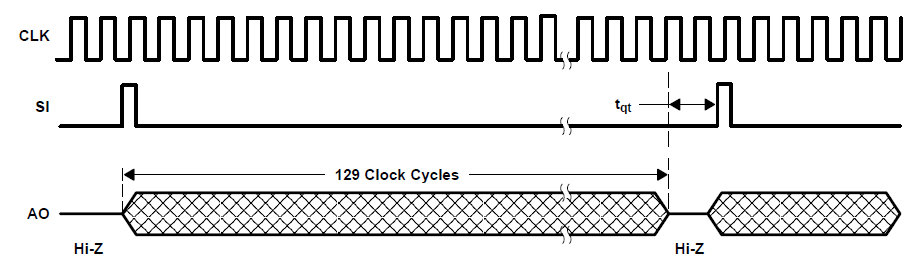
\includegraphics[width=.95\textwidth]{sec7/images/TimingWaveform} 
\centering
\captionsetup{width=.95\textwidth}
\caption[Zeitverlauf eines vollständigen Bildtransfers aus Sicht der Kamera ~\protect\cite{Taos}]{Zeitverlauf eines vollständigen Bildtransfers aus Sicht der Kamera TSL1401R-LF mit der Mindestdauer von 129 Clock-Zyklen und einer Wartezeit von t\textsubscript{qt} (\glqq{}Pixel Charge Transfer Time\grqq{} = min. 20µs)  ~\protect\cite{Taos}}\centering
\label{fig:TimingWaveform}
\end{figure}


\newpage
\subsection{Ablauf einer Bildaufnahme}\label{Sec7Sub2}

Für das Erstellen eines zeitlichen Ablaufs für die Bildaufnahme des Fahrzeugs werden drei Module des Mikrocontrollers verwendet. Für die Nachbildung der zeitlichen Abläufe, die die Kamera benötigt (SI, CLK), wird der SCTimer des Controllers eingesetzt. Für diesen kann eine Vielzahl von Events konfiguriert werden. Jedes dieser Events kann andere Controller-Module triggern oder Ausgänge des Controllers setzen oder rücksetzen. Das zweite Modul, welches verwendet wird, ist der Analog-Digital-Wandler (ADC). Mithilfe dessen werden die Spannungspegel des analogen Ausgangs der Kamera gemessen. Diese Spannungen repräsentieren die Helligkeiten der einzelnen Pixel. Das dritte eingesetzte Modul ist ein einfacher Timer, der die Bildaufnahmerate festlegt. Die Bildaufnahmerate ist die Frequenz, mit der neue Bilder aufgenommen werden und ist nicht zu verwechseln mit der Bildaufnahmegeschwindigkeit eines einzelnen Bildes!\vspace{11pt}

Abbildung \ref{fig:CAMProcedure} zeigt den zeitlichen Verlauf einer Bildaufnahme aus Sicht des Controllers mit den in dieser Fahrzeugversion festgelegten Zeiten und Events. Event 0 und 1 sind für die Erstellung des Kamera-Clock-Signals zuständig (Event 0: Set CAM\_CLK / Event 1: Clear CAM\_CLK). Die Events 2 (Set CAM\_SI) und 3(Clear CAM\_SI) legen die Relativposition des SI-Signals zur Clock fest. Das Rücksetzen des SI-Signals erfolgt immer, während das Setzen nur dann erlaubt wird, wenn der Timer, der für die Bildaufnahmerate zuständig ist, einen Interrupt auslöst. Das Event 4 triggert den ADC, welcher spätestens bis zum nächsten Trigger-Event ein fertiges Ergebnis geliefert haben muss. Der ADC misst die Spannung an CAM\_AO in jedem Clock-Zyklus. Die Speicherung der Werte erfolgt allerdings nur dann, wenn gerade eine Aufnahme getätigt wird, also insgesamt 128 mal nach dem Erscheinen des SI-Signals.

\begin{figure}[H] %H für Positionierung hier
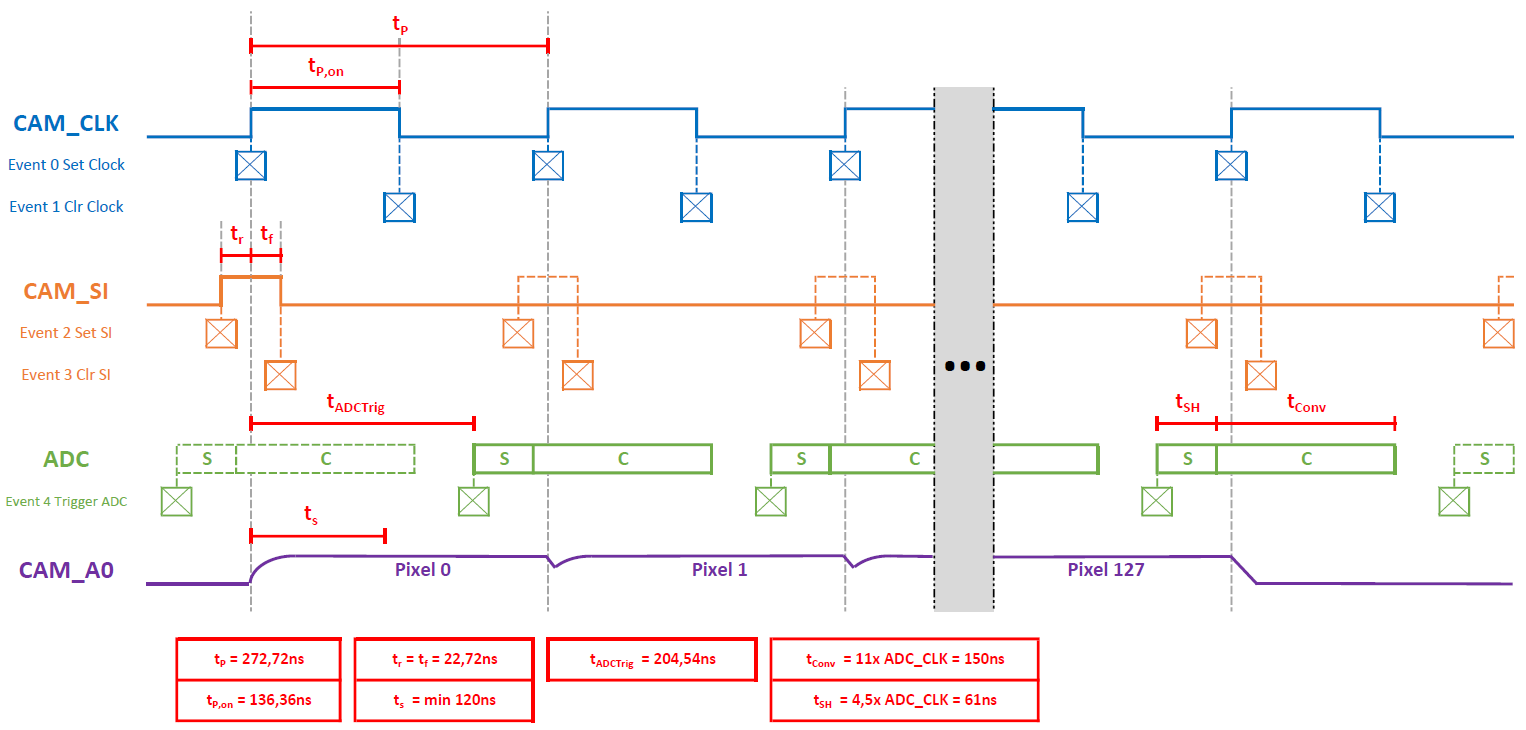
\includegraphics[width=\textwidth]{sec7/images/CAMProcedure} 
\centering
\captionsetup{width=.95\textwidth}
\caption[Zeitlicher Ablauf einer einzelnen Bildaufnahme aus Sicht des Controllers]{Zeitlicher Ablauf einer einzelnen Bildaufnahme aus Sicht des Controllers}\centering
\label{fig:CAMProcedure}
\end{figure}

\newpage

\subsection{Programmierung der zyklischen Bildaufnahme}\label{Sec7Sub3}

Der gesamte Code für die Inbetriebnahme der Kamera ist wie bei der Servo-Lenkung und bei den Antrieben in zwei Dateien unterteilt. In der Datei \glqq{}camera.h\grqq{} befinden sich die Funktionsprototypen und die Einbindung der für die Kamera notwendigen Bibliotheken (Prototypen siehe Abbildung \ref{fig:camh}). Die Datei \glqq{}camera.c\grqq{} enthält hingegen die gesamten Funktionen, die für die Realisierung der zyklischen Bildaufnahme notwendig sind und im Folgenden näher erläutert werden.

\begin{figure}[H] %H für Positionierung hier
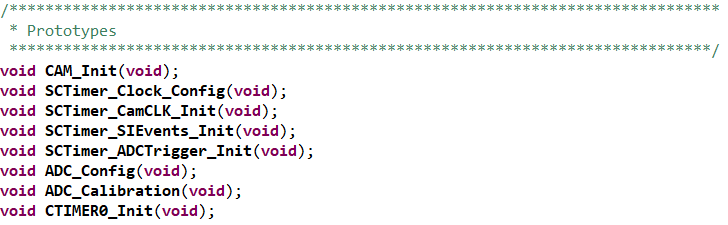
\includegraphics[width=.95\textwidth]{sec7/images/code/camerah} 
\centering
\captionsetup{width=.95\textwidth}
\caption[Prototypen der Kamerafunktionen in der Datei \glqq{}camera.h\grqq{}]{Prototypen der Kamerafunktionen aus \glqq{}camera.c\grqq{} in der Datei \glqq{}camera.h\grqq{}}\centering
\label{fig:camh}
\end{figure}


%***********************************************************************************
% CAM_Init
%***********************************************************************************
Die Primärfunktion der Kamera-Initialisierung (\glqq{}CAM\_Init\grqq{}, siehe Abbildung \ref{fig:CAMInit}) ruft aus Übersichtlichkeitsgründen lediglich alle anderen notwendigen Initialisierungs- und Konfigurationsfunktionen auf und startet an ihrem Ende den SCTimer SCT0, welcher die Clock-Events, SI-Events und das ADC-Trigger-Event generiert.

\begin{figure}[H] %H für Positionierung hier
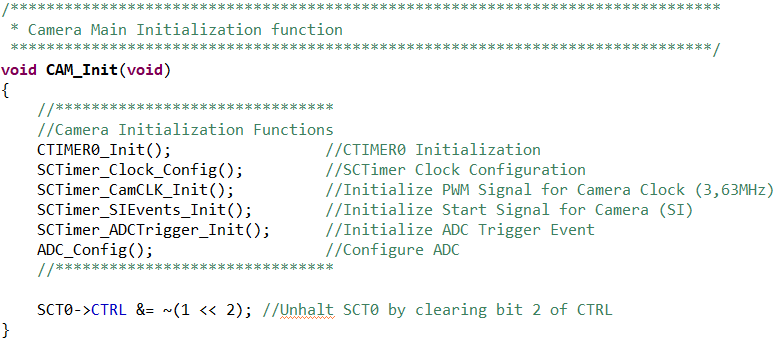
\includegraphics[width=.95\textwidth]{sec7/images/code/CAMInit} 
\centering
\captionsetup{width=.95\textwidth}
\caption[Funktion \glqq{}CAM\_Init\grqq{} aus der Datei \glqq{}camera.c\grqq{}]{Funktion \glqq{}CAM\_Init\grqq{} als primäre Einstiegsfunktion zur Kamera-Initialisierung; Teil der Datei \glqq{}camera.c\grqq{}}\centering
\label{fig:CAMInit}
\end{figure}

%***********************************************************************************
% CTIMER0_Init
%***********************************************************************************
Die erste Modul-Initialisierung, die in der Funktion \glqq{}CAM\_Init\grqq{} von statten geht, ist die des CTIMER0 (\glqq{}CTIMER0\_Init\grqq{}, siehe Abbildung \ref{fig:CTIMER0Init}). Das Timer-Modul CTIMER0 ist, wie bereits erwähnt, für die Bildaufnahmerate verantwortlich. Zuerst wird festgelegt, was bei einem Timer-Überlauf passieren soll. Bei einem Überlauf, also dann, wenn der Wert des Timer-Zählers gleich dem Wert aus dem Match Register 0 ist, wird sowohl ein Interrupt Request gestartet, der Zähler des Timers auf 0 gesetzt und ein neuer Wert für das Match Register 0 aus dem Shadow Register geladen. Außerdem wird in der Initialisierungsfunktion des Timers die Interrupt Service Routine für das Timer Modul CTIMER0 aktiviert und der Timer gestartet.

\begin{figure}[H] %H für Positionierung hier
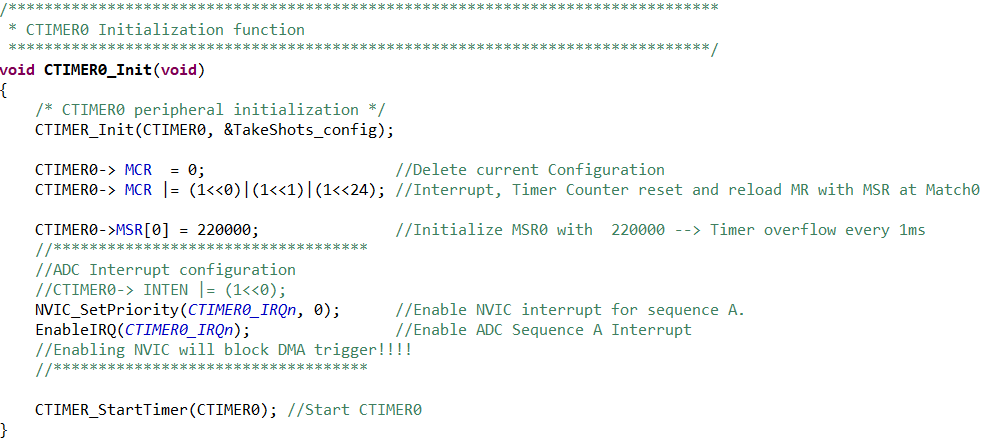
\includegraphics[width=\textwidth]{sec7/images/code/CTIMER0Init} 
\centering
\captionsetup{width=.95\textwidth}
\caption[Funktion \glqq{}CTIMER0\_Init\grqq{} aus der Datei \glqq{}camera.c\grqq{}]{Funktion \glqq{}CTIMER0\_Init\grqq{} für die Initialisierung des Timer Moduls CTIMER0, welches für die Bildaufnahmerate zuständig ist; Teil der Datei \glqq{}camera.c\grqq{}}\centering
\label{fig:CTIMER0Init}
\end{figure}

Bei einer Bildaufnahme in regelmäßigen Abständen gibt es einen problematischen Effekt, der die Pixelwerte betrifft. Da die Strecke nie gleichmäßig beleuchtet ist, schwankt die durchschnittliche Helligkeit des Bildes erheblich. Wenn zu lange belichtet wird, kann es sogar zu einer Überhöhung der Spannung einiger Pixel kommen, was zu falschen Ergebnissen bei allen Pixeln führt. In beiden Fällen ist die Dauer der Belichtung ungünstig gewählt. Um diesem Problem entgegenzuwirken muss die Belichtungszeit angepasst werden und das am besten nach jeder Aufnahme. Belichtet wird bei der Kamera immer dann, wenn nicht gerade eine Aufnahme getätigt wird. Um die Belichtungszeit anzupassen, muss also lediglich der Überlaufwert des Timers im Shadow Register verändert werden (Anpassung der Regelmäßigkeit des die Kamera startenden SI-Events). Da aus Zeitgründen die Anpassung der Belichtungszeit nicht mehr implementiert werden konnte, ist im Folgenden der theoretisch erarbeitete Ablauf der Belichtungszeitanpassung aufgeführt.\vspace{18pt}

\textbf{\underline{Ablauf der Belichtungszeitanpassung nach jeder Aufnahme:}} 
\begin{itemize}
\item Abzählen der hellen und dunklen Pixel\\
	Schwelle hell/dunkel bei 8bit ADC-Auflösung ist 256/2 = 128
\item Gewichten der Pixelwerte\\
	Gewichtung so, dass gleich viele Helligkeitswerte von dunklen und hellen Pixeln in die Mittelwertbestimmung einfließen
\item Mittlere Helligkeit des Bildes berechnen\\
	Addition aller Werte und Bildung des Gradienten mit der Werteanzahl (Werteanzahl variiert je nach Gewichtung)
\item Erörterung, ob bei der nächsten Aufnahme länger oder kürzer belichtet werden muss\\
	Wenn errechnete mittlere Helligkeit höher als 128 --> Belichtungszeit verkürzen\\
	Wenn errechnete mittlere Helligkeit niedriger als 128 --> Belichtungszeit verlängern
\item Anpassung des Überlauf-Werts des Timers CTIMER0 im Shadow Register von Match 0\vspace{18pt}
\end{itemize}

%%***********************************************************************************
%% SCTimer_Clock_Config
%%***********************************************************************************
Im Anschluss an die Initialisierung des Timers CTIMER0 wird in \glqq{}CAM\_Init\grqq{} die Funktion \glqq{}SCTimer\_Clock\_Config\grqq{} aufgerufen (siehe Abbildung \ref{fig:SCTClockConfig}). Darin wird die Clock für den SCTimer SCT0 mit einer Frequenz von 44MHz festgelegt. Die maximale Clock Frequenz für den SCTimer beträgt zwar 100MHz, jedoch reicht die Zeitauflösung bei 44MHz leicht für die Genauigkeit der Zeiteinstellung der einzelnen Events.

\begin{figure}[H] %H für Positionierung hier
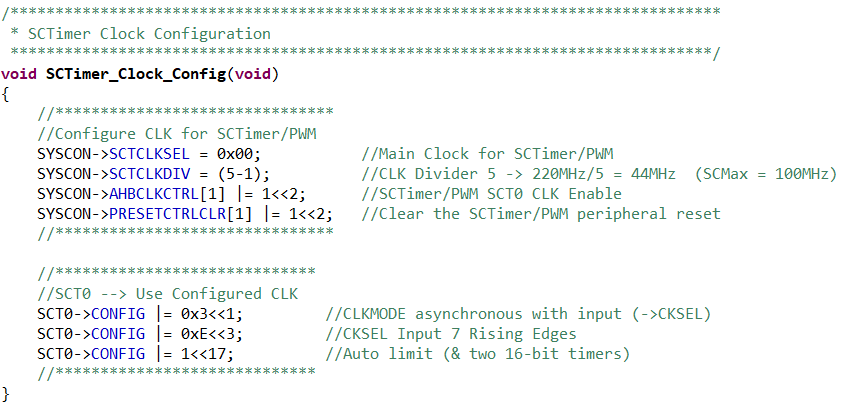
\includegraphics[width=\textwidth]{sec7/images/code/SCTimerClockConfig} 
\centering
\captionsetup{width=.95\textwidth}
\caption[Funktion \glqq{}SCTimer\_Clock\_Config\grqq{} aus der Datei \glqq{}camera.c\grqq{}]{Funktion \glqq{}SCTimer\_Clock\_Config\grqq{} für die Konfiguration der Modul-Clock des SCTimers; Teil der Datei \glqq{}camera.c\grqq{}}\centering
\label{fig:SCTClockConfig}
\end{figure}

%%***********************************************************************************
%% SCTimer_CamCLK_Init
%%***********************************************************************************
Als nächstes wird mit der Funktion \glqq{}SCTimer\_CamCLK\_Init\grqq{} das Kamera-Clock Signal erstellt (siehe Abbildung \ref{fig:SCTimerCamCLKInit}), also die Events 0 und 1 konfiguriert. Die Clock wird mithilfe des SCTimer-Ausgangs SCT0\_OUT1 am Pin 13 der Buchsenleiste J13 nach außen geführt (Port-Pin P3.27). Das Event 0 setzt den Ausgang, während das Event 1 den Ausgang zurücksetzt. Um mit dem ADC eine 8 bit Auflösung zu erreichen, kann die Kamera-Clock nicht mit der technischen Grenze von 8MHz betrieben werden. Deshalb wird die Frequenz auf 3,63MHz festgesetzt. Das entspricht einer Periodendauer von 272,72ns (Event 0) und einer On-Zeit von 136,36ns (Event 1). Beide Events sind immer aktiv, die Kamera-Clock läuft also die ganze Zeit durch.\vspace{11pt}


\begin{figure}[H] %H für Positionierung hier
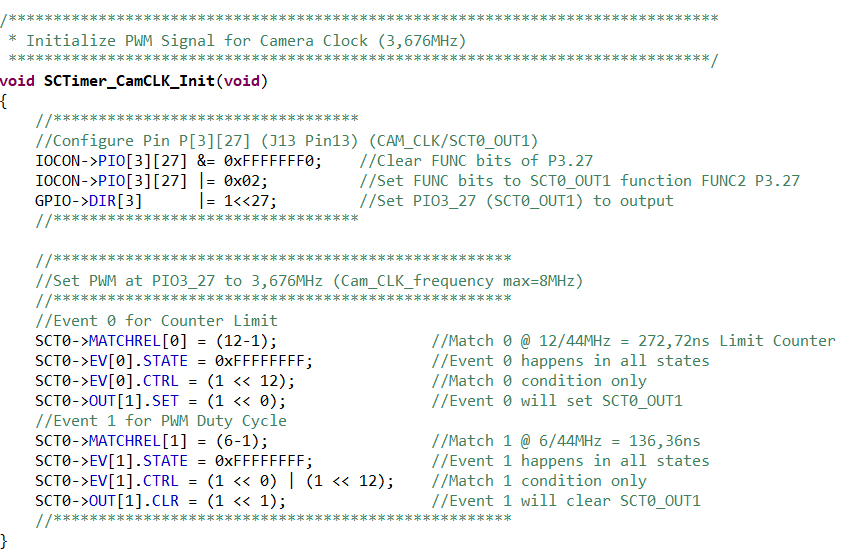
\includegraphics[width=.95\textwidth]{sec7/images/code/SCTimerCamCLKInit} 
\centering
\captionsetup{width=.95\textwidth}
\caption[Funktion \glqq{}SCTimer\_CamCLK\_Init\grqq{} aus der Datei \glqq{}camera.c\grqq{}]{Funktion \glqq{}SCTimer\_CamCLK\_Init\grqq{} für die Initialisierung der Events für die Kamera-Clock; Teil der Datei \glqq{}camera.c\grqq{}}\centering
\label{fig:SCTimerCamCLKInit}
\end{figure}

%%***********************************************************************************
%% SCTimer_SIEvents_Init
%%***********************************************************************************

Um die Bildaufnahme starten zu können, muss mit dem seriellen Eingang der Kamera die Bildaufnahme getriggert werden, was über die Events 2 und 3 des SCTimers realisiert wird. Diese Events werden in der Funktion \glqq{}SCTimer\_SIEvents\_Init\grqq{} initialisiert (siehe Abbildung \ref{fig:SCTimerSIEventsInit}). Wie bereits erwähnt, muss das Setzen des SI-Ausgangs, welcher über den SCTimer-Ausgang SCT0\_OUT0 am Pin 15 der Buchsenleiste J13 nach außen geführt ist (Port-Pin P3.26), mindestens 20ns vor der steigenden Flanke der Kamera-Clock erfolgen (Event 2, Set CAM\_SI). Das Rücksetzen des SI-Signals könnte theoretisch auch mit dem Event 0 (Set CAM\_CLK) erfolgen. Da im SCTimer allerdings noch genügend Events zur Verfügung stehen, wird das Event 3 (Clear CAM\_SI) so eingestellt, dass das SI-Signal mit der gleichen Zeit nach der steigenden Flanke der Clock zurückgesetzt wird, mit der es vor der steigenden Flanke gesetzt wurde. Deshalb wird für das Event 2 eine Zeit von 250ns (250ns - 272,72ns = -22,72ns) und für das Event 3 eine Zeit von 22,72ns eingestellt.\vspace{11pt}

Das Event 3 wird in jedem Zyklus ausgeführt, während das Event 2 zum Setzen des SI-Signals in der Interrupt Service Routine des Timers CTIMER0 nur zyklisch erlaubt wird. Deshalb wird für das Event 2 im EV[2].State Register nicht 0xFFFFFFF (Event wird in jedem Status ausgelöst) sondern 0 eingetragen (Auslösung des Events nur in Status 0). Da der Status während des Betriebs des SCTimers in dieser Anwendungsform nie verändert wird, wirkt eine 0 im Status Register wie eine vollständige Deaktivierung des Events, die in der Interrupt Service Routine des Timers kurzzeitig für ein einmaliges Auslösen aufgehoben wird. Der zyklische Eintritt in die Interrupt Service Routine legt daher die Bildaufnahmerate fest.

\begin{figure}[H] %H für Positionierung hier
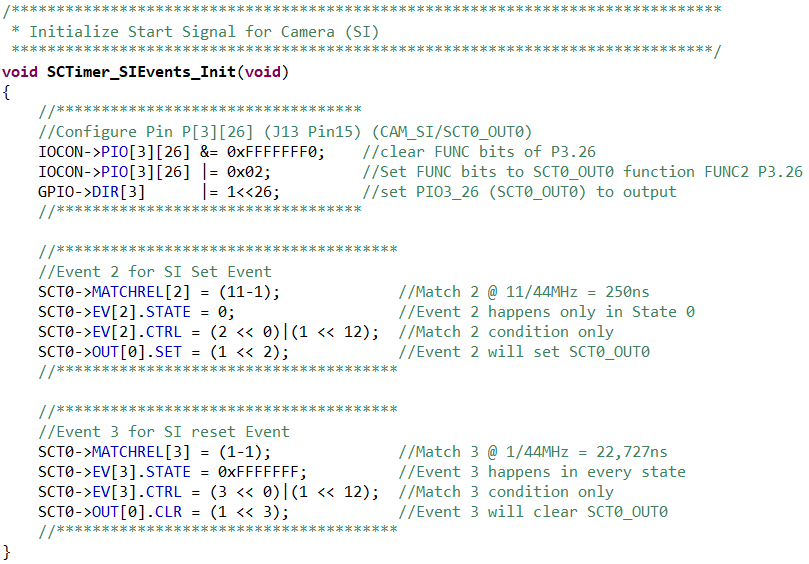
\includegraphics[width=.95\textwidth]{sec7/images/code/SCTimerSIEventsInit} 
\centering
\captionsetup{width=.95\textwidth}
\caption[Funktion \glqq{}SCTimer\_SIEvents\_Init\grqq{} aus der Datei \glqq{}camera.c\grqq{}]{Funktion \glqq{}SCTimer\_SIEvents\_Init\grqq{} für die Initialisierung der Events für den seriellen Eingang der Kamera; Teil der Datei \glqq{}camera.c\grqq{}}\centering
\label{fig:SCTimerSIEventsInit}
\end{figure}

%%***********************************************************************************
%% CTIMER0_IRQHandler
%%***********************************************************************************

\begin{figure}[H] %H für Positionierung hier
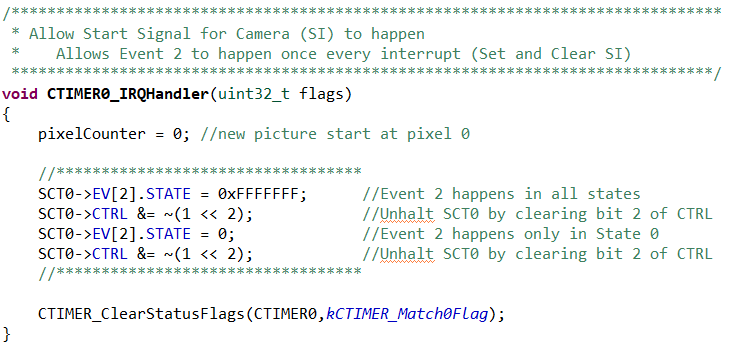
\includegraphics[width=.95\textwidth]{sec7/images/code/CTIMER0IRQHandler} 
\centering
\captionsetup{width=.95\textwidth}
\caption[Interrupt Service Routine \glqq{}CTIMER0\_IRQHandler\grqq{} aus der Datei \glqq{}camera.c\grqq{}]{Interrupt Service Routine \glqq{}CTIMER0\_IRQHandler\grqq{} für die kurzzeitige Aktivierung des Events 2 (Set CAM\_SI) und das Rücksetzen der Pixel Zähler-Variable; Teil der Datei \glqq{}camera.c\grqq{}}\centering
\label{fig:CTIMER0IRQHandler}
\end{figure}

Wird bei einem Timer Überlauf des Timers CTIMER0 ein Interrupt Request ausgelöst, wird daraufhin die Interrupt Service Routine \glqq{}CTIMER0\_IRQHandler\grqq{} ausgeführt (siehe Abbildung \ref{fig:CTIMER0IRQHandler}). In ihr wird nicht nur das Event 2 kurzfristig aktiviert, sondern auch der Pixel-Zähler zurückgesetzt, damit bei einer neuen Bildaufnahme die vom ADC aufgenommenen Spannungswerte wieder den zugehörigen Pixeln zugeordnet werden kann. Die Häufigkeit des Eintretens in die Interrupt Service Routine wird durch den Überlaufwert des Timers CTIMER0 im Match Register 0 festgelegt und beeinflusst direkt die Belichtungsdauer.\vspace{11pt}


%%***********************************************************************************
%% SCTimer_ADCTrigger_Init
%%***********************************************************************************

Zuletzt muss der SCTimer auch die Aufgabe des ADC-Triggers erfüllen. Die Initialisierung des dafür zuständigen Event 4 wird in der Funktion \glqq{}SCTimer\_ADCTrigger\_Init\grqq{} realisiert (siehe Abbildung \ref{fig:SCTimerADCTriggerInit}). Anders als die SCTimer-Ausgänge SCT0\_OUT0 (CAM\_SI) und SCT0\_OUT1 (CAM\_CLK) wird der ADC-Trigger (SCT0\_OUT4) nicht auf einen Pin nach Außen geführt, sondern lediglich der ADC so konfiguriert, dass der SCTimer Ausgang SCT0\_OUT4 als Hardware Trigger für den ADC verwendet wird.

\begin{figure}[H] %H für Positionierung hier
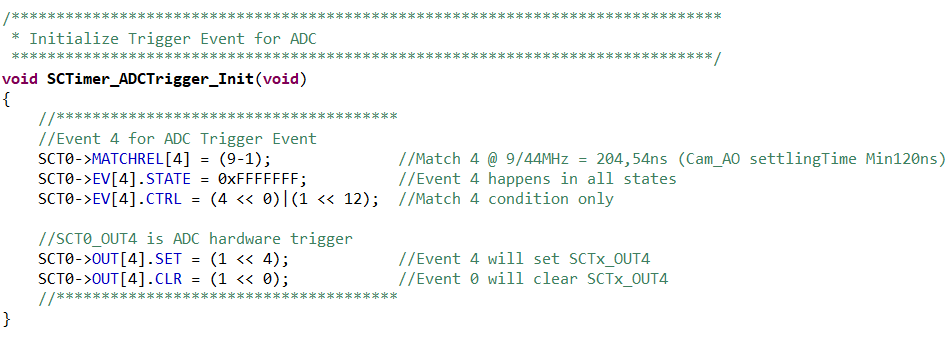
\includegraphics[width=.95\textwidth]{sec7/images/code/SCTimerADCTriggerInit} 
\centering
\captionsetup{width=.95\textwidth}
\caption[Funktion \glqq{}SCTimer\_ADCTrigger\_Init\grqq{} aus der Datei \glqq{}camera.c\grqq{}]{Funktion \glqq{}SCTimer\_ADCTrigger\_Init\grqq{} für die Initialisierung des Events für den Start einer ADC-Konversion; Teil der Datei \glqq{}camera.c\grqq{}}\centering
\label{fig:SCTimerADCTriggerInit}
\end{figure}

%%***********************************************************************************
%% ADC_Config
%%***********************************************************************************
Nach der Konfiguration der Module SCT0 und CTIMER0 muss lediglich noch der ADC konfiguriert werden (Funktion \glqq{}ADC\_Config\grqq{}, siehe Abbildung \ref{fig:ADCConfig}). Als Messeingang für das Analogsignal der Kamera (CAM\_AO) wird der ADC-Eingang ADC0IN4 verwendet (J12 Pin2, Port-Pin P0.16). Zuerst wird die ADC Peripherie aktiviert und die Referenzspannungen eingestellt. Im Anschluss daran wird die Clock für den ADC aktiviert und eine Kalibrierung gestartet (siehe Funktion \glqq{}ADC\_Calibration\grqq{}). Ist die Kalibrierung des ADC zu Ende, wird der ADC mit einer Clock von 73,33MHz initialisiert (max. 80MHz), eine Auflösung von 8bit festgelegt (Wertebereich 0-256) und die Sampling-Zeit eingestellt (hier 4,5x ADC Clock Cycle = 61,26ns). Die Konversionszeit beträgt dann für eine 8bit Auflösung $(11 + 4,5) \cdot ADC_{CLKCycle}$, also insgesamt 211ns. Im Anschluss daran wird noch die Trigger-Quelle auf SCT0\_OUT4 festgelegt und die Interrupt Service Routine des ADC für jede fertige Konversion aktiviert.

\begin{figure}[H] %H für Positionierung hier
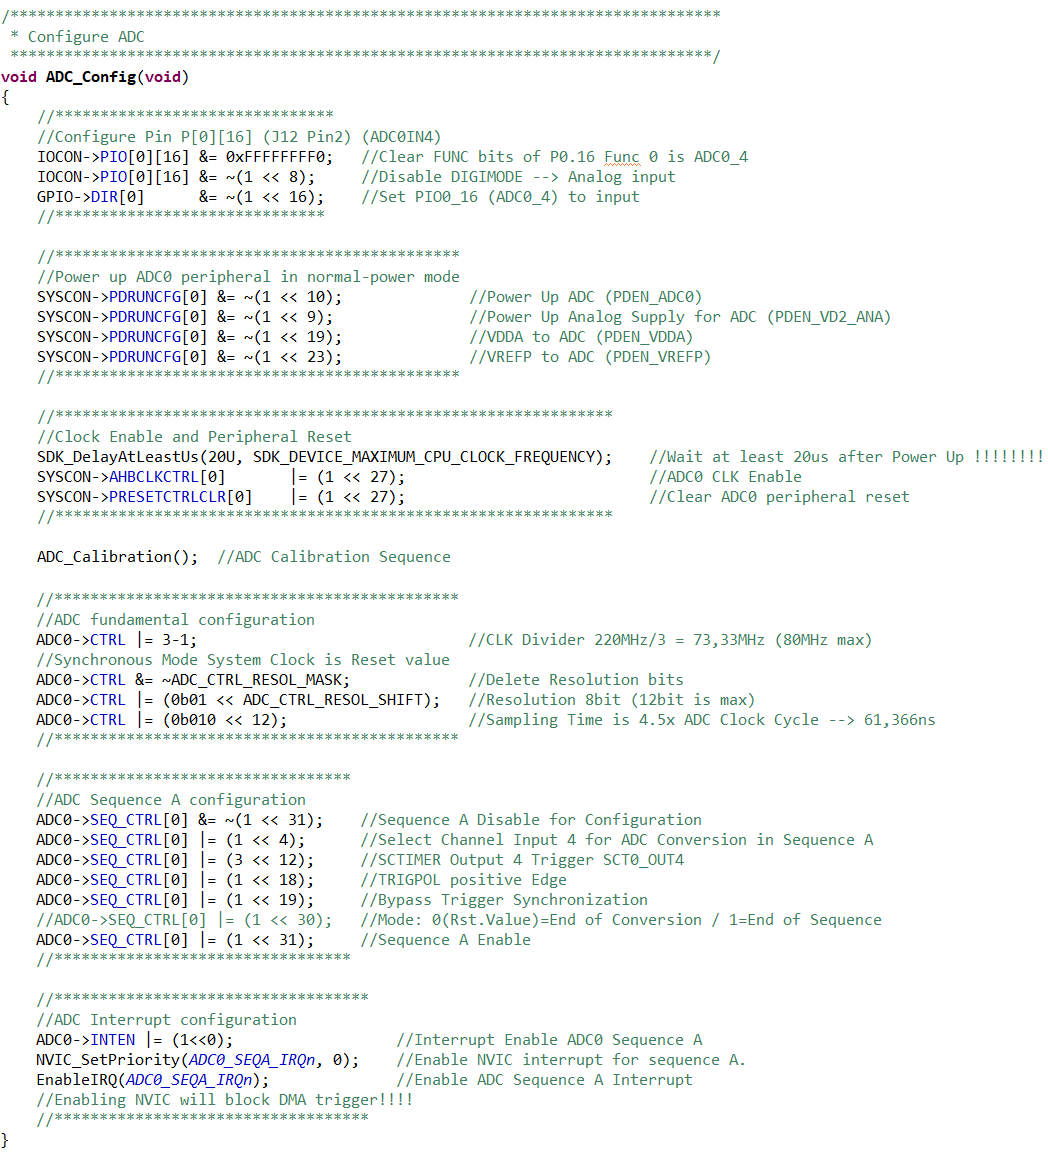
\includegraphics[width=.95\textwidth]{sec7/images/code/ADCConfig} 
\centering
\captionsetup{width=.95\textwidth}
\caption[Funktion \glqq{}ADC\_Config\grqq{} aus der Datei \glqq{}camera.c\grqq{}]{Funktion \glqq{}ADC\_Config\grqq{} für die Konfiguration des Analog-Digital-Wandlers; Teil der Datei \glqq{}camera.c\grqq{}}\centering
\label{fig:ADCConfig}
\end{figure}

%%***********************************************************************************
%% ADC_Calibration
%%***********************************************************************************

Die ADC-Kalibrierung folgt einem festen Ablauf. Damit es egal ist, wann die Kalibrierfunktion \glqq{}ADC\_Calibration\grqq{} (siehe Abbildung \ref{fig:ADCCalibration})aufgerufen wird, wird zuerst die aktuelle Konfiguration gespeichert und am Ende der Kalibrierung diese wieder geladen. Dazwischen wird der Clock-Divider auf unter 30MHz umprogrammiert (Maximale Kalibrierfrequenz) und der Kalibrationszyklus gestartet.\vspace{11pt}

Nach jeder ADC-Konversion wird ein Interrupt Request ausgelöst und die Interrupt Service Routine \glqq{}ADC0\_SEQA\_IRQHandler\grqq{} (siehe Abbildung \ref{fig:ADC0SEQAIRGHandler}) ausgeführt.
In ihr werden die vom ADC ermittelten Werte der Reihe nach mithilfe des Pixel-Zählers, welcher in der Interrupt Service Routine des CTIMER0 beim Start einer Bildaufnahme jedes mal zurückgesetzt wird, in ein Ergebniswert-Array gespeichert (uint8\_t pixelValues[pixelCounter]).

\begin{figure}[H] %H für Positionierung hier
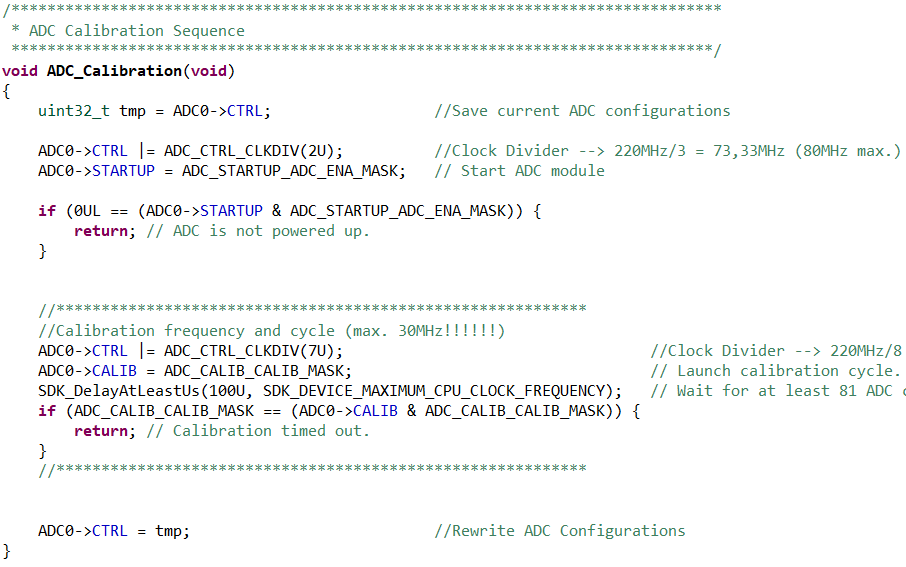
\includegraphics[width=.95\textwidth]{sec7/images/code/ADCCalibration} 
\centering
\captionsetup{width=.95\textwidth}
\caption[Funktion \glqq{}ADC\_Calibration\grqq{} aus der Datei \glqq{}camera.c\grqq{}]{Funktion \glqq{}ADC\_Calibration\grqq{} für die Konfiguration des Analog-Digital-Wandlers; Teil der Datei \glqq{}camera.c\grqq{}}\centering
\label{fig:ADCCalibration}
\end{figure}

%%***********************************************************************************
%% ADC0_SEQA_IRQHandler
%%***********************************************************************************

\begin{figure}[H] %H für Positionierung hier
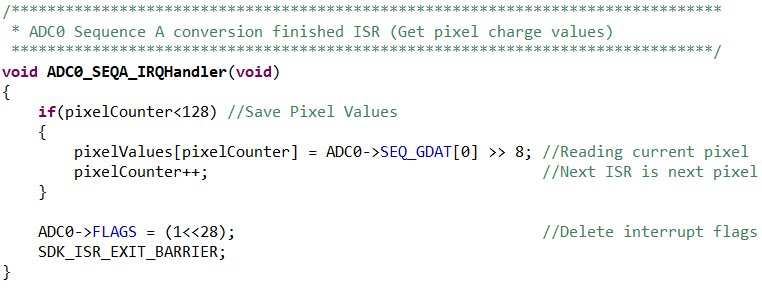
\includegraphics[width=.95\textwidth]{sec7/images/code/ADC0SEQAIRQHandler} 
\centering
\captionsetup{width=.95\textwidth}
\caption[Interrupt Service Routine \glqq{}ADC0\_SEQA\_IRQHandler\grqq{} aus der Datei \glqq{}camera.c\grqq{}]{Interrupt Service Routine \glqq{}ADC0\_SEQA\_IRQHandler\grqq{} für die Ergebniswertaufnahme nach jeder ADC-Konversion; Teil der Datei \glqq{}camera.c\grqq{}}\centering
\label{fig:ADC0SEQAIRGHandler}
\end{figure}

%%***********************************************************************************
%% Calculation
%%***********************************************************************************

Aus den vom ADC gemessenen Werten können mit dem Algorithmus aus Abbildung \ref{fig:PixelCalc} am Ende einer Bildaufnahme sowohl der reelle Spannungswert, als auch der logische Wert für Hell oder Dunkel bestimmt werden. Da mit den 8bit Werten eine Regelung qualitativ genauso gut realisierbar ist, wie mit Spannungswerten, ist der Algorithmus lediglich zu Testzwecken in der Datei \glqq{}camera.c\grqq{} eingebunden.

\begin{figure}[H] %H für Positionierung hier
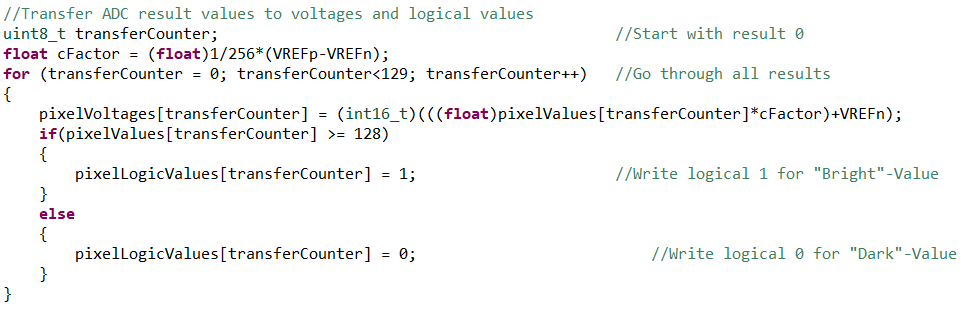
\includegraphics[width=.95\textwidth]{sec7/images/code/PixelCalc} 
\centering
\captionsetup{width=.95\textwidth}
\caption[Algorithmus für die Bestimmung der Spannungswerte und logischen Werte der Pixel]{Algorithmus für die Bestimmung der Spannungswerte und logischen Werte der Pixel aus den vom ADC bestimmten 8bit Werten}\centering
\label{fig:PixelCalc}
\end{figure}

Außer der bisher verwendeten Module (ADC0, SCTIMER0, CTIMER0) kann es auch sinnvoll sein, den Direct Memory Access (DMA) für die Ergebnisse des ADCs zu verwenden. Ein Direktzugriff des ADC auf den Speicher spart Rechenressourcen und Zeit, was die maximal mögliche Bildaufnahmerate weiter erhöht. Da bisher lediglich die Bildaufnahme realisiert werden konnte, ist es außerdem notwendig, die Aufbereitung der Messergebnisse zu implementieren. Eine Aufbereitung der Messergebnisse ist beispielsweise die automatische Belichtungszeitanpassung oder ein Verrechnung nebeneinanderliegender Pixelwerte für die bessere Erkennung der Fahrbahnbegrenzungen.

%\subsection{Montage und Ausrichtung der Kamera}\label{Sec7Sub4}

%Für die Montage der Kamera wird die 3D-gedruckte Kamera-Halterung aus Kapitel \ref{Sec2Sub2SubSub6} verwendet. Die Halterung lässt zum einen eine individuelle Einstellung der Höhe zu und zum anderen ermöglicht die Verzahnung der Halterung eine individuelle Ausrichtung der Kamera.\vspace{11pt} 

%Da bisher lediglich die Streckenauswertung und noch nicht die Regelung implementiert werden konnte, gibt es noch keine Erfahrungswerte für die optimale Positionierung und Ausrichtung der Kamera am Fahrzeug.

%\subsection{Kameralinsen}\label{Sec7Sub4}
%***CHRIS***

\newpage